\subsection{Analyse der Ergebnisse} \label{analyse-subsec}


Es sei darauf hingewiesen, dass Lösungen, die auf der Verwendung von Deep Neural Networks (DNNs) zur Extraktion von Merkmalen basieren (z.B. Multi-Layer-Perceptron, Convolutional Neural oder Long-Short-Term-Memory Networks) ebenfalls getestet wurden. Diese Ansätze konnten aber nicht so gute Ergebnisse erzielen, wie die handgefertigten Merkmale. Erkennungsraten für die am wenigsten vertretenen Klassen (insbesondere ``Frustration'') scheinen der Grund für die schwache Performance der DNNs zu sein. Wir gehen davon aus, dass dieses Phänomen durch die relativ geringe Größe unseres Datensatzes verursacht wird. \\

Entgegen unserern Erwartungen liefert der CA schächere Performance als die handgefertigten Merkmale. Der Grund hierfür ist aber sehr wahrscheinlich der selbe wie bei den  DNNs, und zwar der relativ kleine Datensatz. 
Eine kleine qualitative Analyse der in der Studie verwendeten Daten kann die Gründe für diese Beobachtungen begründen. 
CA-Merkmale (sowohl für weiche als auch für harte Zuweisungen) sind per Definition sehr empfindlich gegenüber Variationen der Formen der Originalsignale: Die Codewörter werden durch Clustering auf Sätzen von Segmenten bestimmt, die aus den Originalsignalen extrahiert wurden, und die histogrammbasierten Merkmale selbst basieren auf direkten Vergleichen zwischen den Codewörtern und dem Segment der zu klassifizierenden Daten. 
Daher kann jede Quelle von Rauschen oder Unregelmäßigkeiten in den Originaldaten die Effektivität der CA-Funktionen stark beeinträchtigen. 
Ein Blick auf die in unserer Studie verwendeten Signale ergab zwei Hauptprobleme: falsche Datenwerte, die durch Hardwareprobleme bei einigen Sensoren verursacht wurden (wie in Abbildung \ref{fig:bad_signals}), und das Vorhandensein von Rauschen, das Unregelmäßigkeiten in den Signalformen verursacht (siehe Abbildung \ref{fig:zoom}). Mögliche Lösungen zur Behebung dieses Problems könnten sein, zusätzliche Vorverarbeitungstechniken zur Rauschunterdrückung einzusetzen, wie z.B. Tiefpassfilterung. \\


\begin{figure}[h]
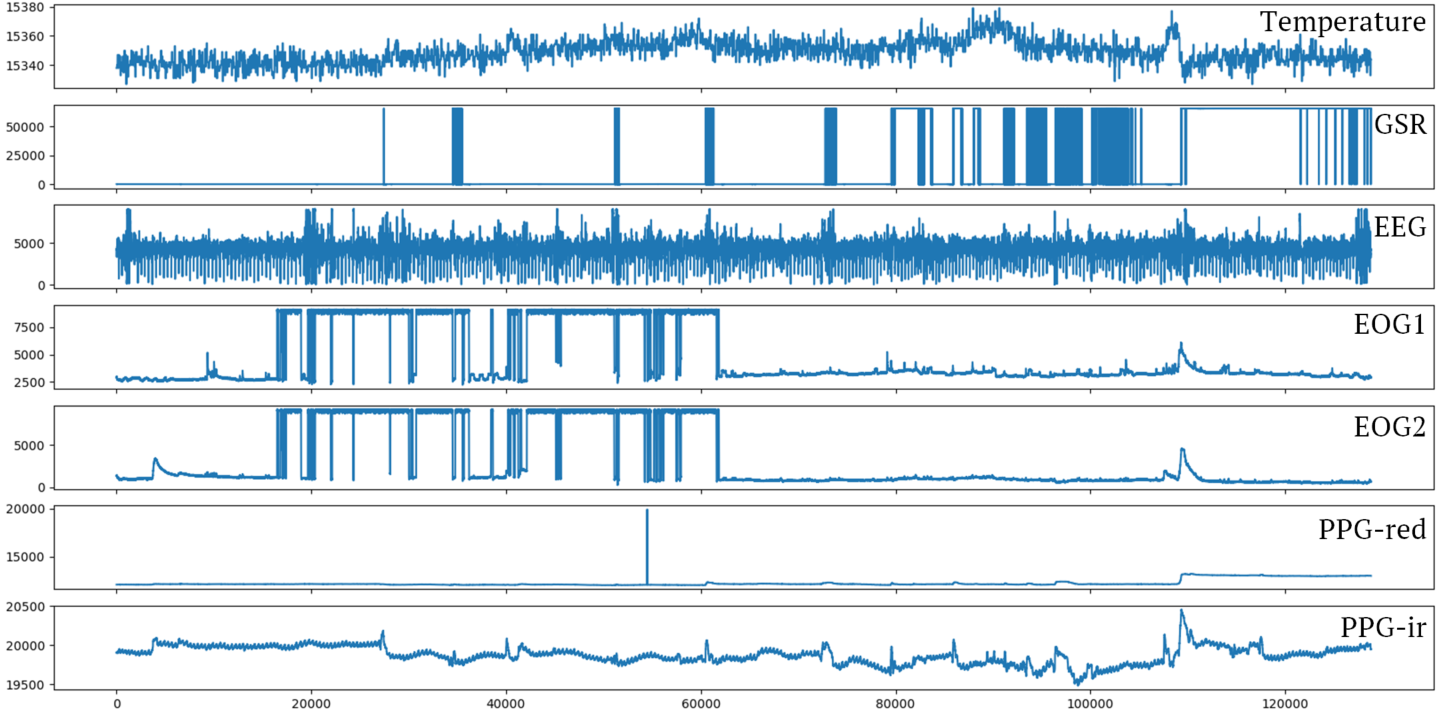
\includegraphics[width=\textwidth]{Images/bad_signals.png} 
\vspace{-0.3cm} \caption[Sensoraufzeichnungen von Daten]{ Sensoraufzeichnungen von Daten, die im Rahmen des ELISE-Projekts von einem der drei getesteten Probanden erfasst wurden. Die x-Achse repräsentiert die Zeit und die y-Achse die Sensorwerte. Die in den Daten von GSR und den beiden EOG-Kanälen sichtbaren Unregelmäßigkeiten deuten auf Probleme mit der Hardware hin. }
\label{fig:bad_signals} \end{figure} \vspace{0.5cm}


\begin{figure}[h]
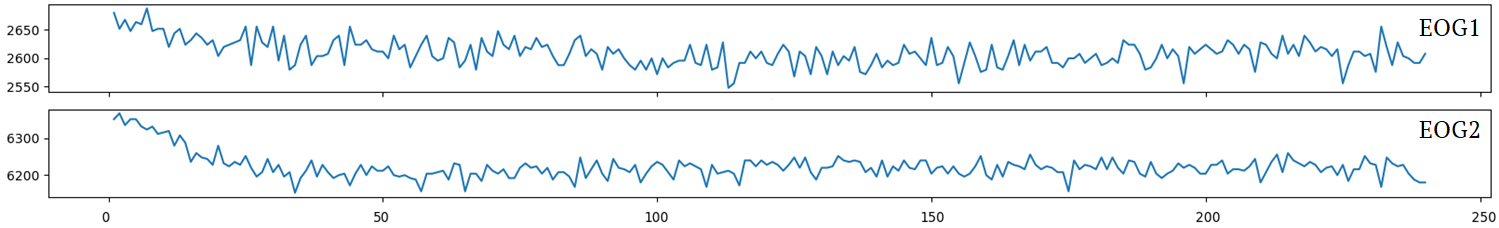
\includegraphics[width=\textwidth]{Images/zoom.png} 
\vspace{-0.3cm} \caption[Nahaufnahme von Rauschen in Daten]{ Nahaufnahme der im Rahmen des ELISE-Projekts erworbenen EOG-Kanäle von einem der drei getesteten Probanden. Das Vorhandensein von Rauschen in den Daten ist sichtbar, das zu Unregelmäßigkeiten in den Signalformen führt. }
\label{fig:zoom} \end{figure} \vspace{0.5cm}



\newpage

Allgemein deuten die Ergebnisse aber darauf hin, dass unser biomedizinisches Datenerfassungssystem zur Emotionserkennung erfolgreich eingesetzt werden könnte, um ein intelligent adaptives Lernsystems zu verbessern. Zukünftige Arbeiten werden die Verfeinerung des Multisensor-Datenerfassungsgerätes, die Erfassung weiterer und größerer Datensätze für die weitere Mustererkennungsanalyse und die Analyse der Wirksamkeit des Emotionserkennungssystems in einem VR-affektiven Lernkontext beinhalten.